% Method schematic for the birth excess/deficit paper.
% Compile standalone:  pdflatex method_schematic.tex
% Or copy the tikzpicture into the manuscript (needs the \usetikzlibrary lines).
\documentclass[tikz,border=6pt]{standalone}
\usepackage{amsmath}
\usetikzlibrary{arrows.meta,calc,positioning}

\usepackage[scaled]{helvet}
\renewcommand{\familydefault}{\sfdefault}

\definecolor{tTeal}{HTML}{1B9E77}
\definecolor{tPurp}{HTML}{7570B3}
\definecolor{tBlue}{HTML}{2C7FB8}
\definecolor{tOrng}{HTML}{E6550D}
\definecolor{tNavy}{HTML}{1A3B5D}
\definecolor{pFill}{HTML}{FBFCFE}
\definecolor{pEdge}{HTML}{C7D2E0}
\definecolor{bFill}{HTML}{EEF3F9}

\begin{document}
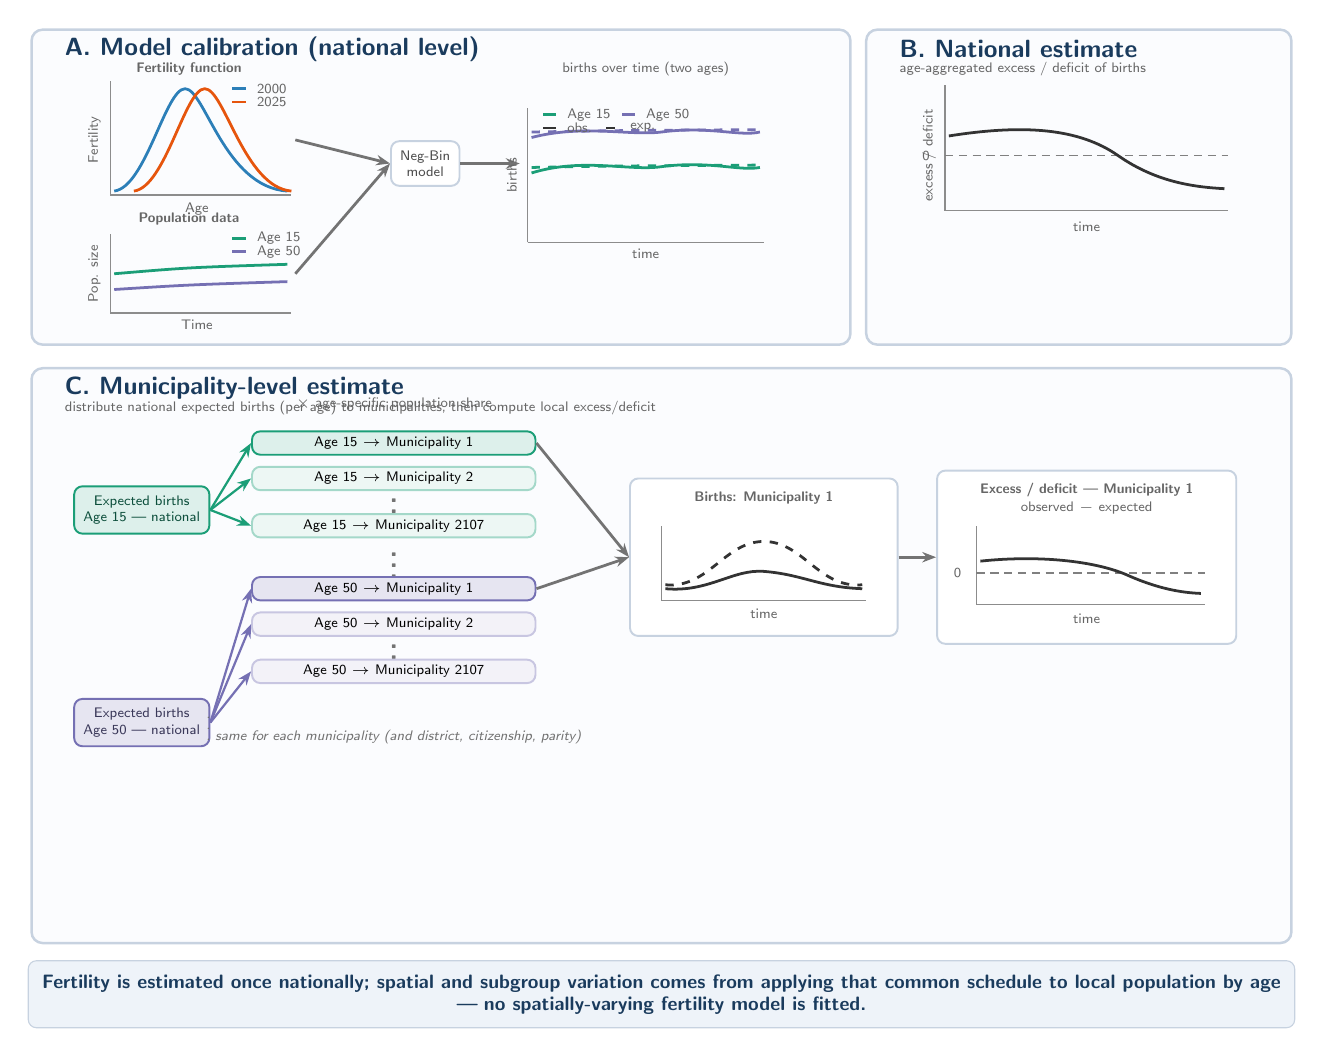
\begin{tikzpicture}[
  font=\sffamily,
  >={Stealth[length=5pt]},
  panel/.style={draw=pEdge,fill=pFill,rounded corners=4pt,line width=.9pt},
  box/.style={draw=pEdge,fill=white,rounded corners=3pt,line width=.7pt},
  row/.style={box,font=\tiny,minimum width=3.6cm,inner sep=2pt},
  vd/.style={font=\bfseries,text=black!55},
  ptitle/.style={font=\small\bfseries,text=tNavy},
  sub/.style={font=\tiny,text=black!60},
  ax/.style={black!45,line width=.5pt},
  teal/.style={draw=tTeal,line width=1pt},
  purp/.style={draw=tPurp,line width=1pt},
  blue/.style={draw=tBlue,line width=1pt},
  orng/.style={draw=tOrng,line width=1pt},
  obs/.style={black!80,line width=1pt},
  exp/.style={black!80,line width=1pt,dashed},
  flow/.style={->,draw=black!55,line width=1pt},
  zero/.style={black!50,line width=.5pt,densely dashed},
  transform shape
]

% =================================================== PANEL A (top-left)
\draw[panel] (0,8.7) rectangle (10.4,12.7);
\node[ptitle,anchor=west] at (0.3,12.45) {A. Model calibration (national level)};

% A1 fertility by age
\node[sub,font=\tiny\bfseries] at (2.0,12.2) {Fertility function};
\draw[ax] (1.0,10.6)--(3.3,10.6);
\draw[ax] (1.0,10.6)--(1.0,12.05);
\draw[blue] (1.05,10.65) .. controls (1.45,10.7) and (1.7,11.95) .. (1.95,11.95)
                         .. controls (2.2,11.95) and (2.45,10.7) .. (3.25,10.65);
\draw[orng] (1.3,10.65)  .. controls (1.7,10.7) and (1.95,11.95) .. (2.2,11.95)
                         .. controls (2.45,11.95) and (2.7,10.7) .. (3.3,10.65);
\node[sub] at (2.1,10.42) {Age};
\node[sub,rotate=90] at (0.8,11.3) {Fertility};
\draw[blue] (2.55,11.95)--(2.72,11.95); \node[sub,anchor=west] at (2.74,11.95){2000};
\draw[orng] (2.55,11.78)--(2.72,11.78); \node[sub,anchor=west] at (2.74,11.78){2025};

% A2 population over time (two ages)
\node[sub,font=\tiny\bfseries] at (2.0,10.3) {Population data};
\draw[ax] (1.0,9.1)--(3.3,9.1);
\draw[ax] (1.0,9.1)--(1.0,10.1);
\draw[teal] (1.05,9.6) .. controls (2.0,9.68) .. (3.25,9.72);
\draw[purp] (1.05,9.4) .. controls (2.0,9.46) .. (3.25,9.5);
\draw[teal] (2.55,10.05)--(2.72,10.05);\node[sub,anchor=west] at (2.74,10.05){Age 15};
\draw[purp] (2.55,9.88)--(2.72,9.88); \node[sub,anchor=west] at (2.74,9.88){Age 50};
\node[sub] at (2.1,8.95) {Time};
\node[sub,rotate=90] at (0.8,9.6) {Pop. size};

% model box
\node[box,align=center,font=\tiny,text=black!70] (model) at (5.0,11.0) {Neg-Bin\\model};
\draw[flow] (3.35,11.3) -- (model.west);
\draw[flow] (3.35,9.6)  -- (model.west);

% A3 births over time (two ages, obs centred on exp)
\node[sub] at (7.8,12.2) {births over time (two ages)};
\draw[flow] (model.east) -- (6.2,11.0);
\draw[ax] (6.3,10.0)--(9.3,10.0);
\draw[ax] (6.3,10.0)--(6.3,11.7);
\draw[teal,dashed] (6.35,10.95) .. controls (7.5,10.97) .. (9.25,10.98);
\draw[teal]        (6.35,10.88) .. controls (7.0,11.08) and (7.6,10.9).. (8.0,10.96)
                                .. controls (8.6,11.04) and (9.0,10.9)..(9.25,10.95);
\draw[purp,dashed] (6.35,11.4)  .. controls (7.5,11.42) .. (9.25,11.43);
\draw[purp]        (6.35,11.33) .. controls (7.0,11.5) and (7.6,11.35)..(8.0,11.4)
                                .. controls (8.6,11.48) and (9.0,11.34)..(9.25,11.4);
\node[sub] at (7.8,9.85) {time};
\node[sub,rotate=90] at (6.1,10.85) {births};
\draw[teal] (6.5,11.62)--(6.66,11.62);\node[sub,anchor=west] at (6.68,11.62){Age 15};
\draw[purp] (7.5,11.62)--(7.66,11.62);\node[sub,anchor=west] at (7.68,11.62){Age 50};
\draw[obs] (6.5,11.45)--(6.66,11.45);\node[sub,anchor=west] at (6.68,11.45){obs.};
\draw[exp] (7.3,11.45)--(7.46,11.45);\node[sub,anchor=west] at (7.48,11.45){exp.};

% =================================================== PANEL B (top-right)
\draw[panel] (10.6,8.7) rectangle (16,12.7);
\node[ptitle,anchor=west] at (10.9,12.45) {B. National estimate};
\node[sub,anchor=west] at (10.9,12.2) {age-aggregated excess / deficit of births};
\draw[ax] (11.6,10.4)--(15.2,10.4);
\draw[ax] (11.6,10.4)--(11.6,12.0);
\draw[zero] (11.6,11.1)--(15.2,11.1);
\node[sub,anchor=east] at (11.53,11.1){0};
\draw[obs] (11.65,11.35) .. controls (12.6,11.5) and (13.3,11.45) .. (13.8,11.1)
                         .. controls (14.3,10.75) and (14.8,10.7) .. (15.15,10.68);
\node[sub] at (13.4,10.2){time};
\node[sub,rotate=90] at (11.4,11.1){excess / deficit};

% =================================================== PANEL C (full width, below)
\draw[panel] (0,1.1) rectangle (16,8.4);
\node[ptitle,anchor=west] at (0.3,8.15) {C. Municipality-level estimate};
\node[sub,anchor=west] at (0.3,7.9) {distribute national expected births (per age) to municipalities, then compute local excess/deficit};

% national expected-births-by-age boxes
% nA is the single absolute anchor for panel C; every other box is placed
% relative to a neighbouring box, so the whole grid moves together if nA moves.
\node[box,fill=tTeal!15,draw=tTeal,align=center,font=\tiny,text=tTeal!50!black]
  (nA) at (1.4,6.6) {Expected births\\Age 15 --- national};
\node[box,fill=tPurp!18,draw=tPurp,align=center,font=\tiny,text=tPurp!50!black]
  (nB) at ([yshift=-2.7cm]nA) {Expected births\\Age 50 --- national};

% municipality rows (Age 15 stack, then Age 50 stack), to the right of the national boxes
\node[row,fill=tTeal!15,draw=tTeal]   (ra1) at ([xshift=3.2cm,yshift=0.85cm]nA) {Age 15 $\rightarrow$ Municipality 1};
\node[sub] at ([yshift=0.33cm]ra1.north) {$\times$ age-specific population share};
\node[row,fill=tTeal!8,draw=tTeal!40] (ra2) at ([yshift=-0.45cm]ra1) {Age 15 $\rightarrow$ Municipality 2};
\node[vd] (vda) at ([yshift=-0.32cm]ra2) {$\vdots$};
\node[row,fill=tTeal!8,draw=tTeal!40] (ra3) at ([yshift=-0.28cm]vda) {Age 15 $\rightarrow$ Municipality 2107};
\node[vd] (vmid) at ([yshift=-0.4cm]ra3) {$\vdots$};
\node[row,fill=tPurp!18,draw=tPurp]   (rb1) at ([yshift=-0.4cm]vmid) {Age 50 $\rightarrow$ Municipality 1};
\node[row,fill=tPurp!9,draw=tPurp!40] (rb2) at ([yshift=-0.45cm]rb1) {Age 50 $\rightarrow$ Municipality 2};
\node[vd] (vdb) at ([yshift=-0.32cm]rb2) {$\vdots$};
\node[row,fill=tPurp!9,draw=tPurp!40] (rb3) at ([yshift=-0.28cm]vdb) {Age 50 $\rightarrow$ Municipality 2107};

% distribution arrows (straight)
\draw[->,tTeal,line width=.8pt] (nA.east) -- (ra1.west);
\draw[->,tTeal,line width=.8pt] (nA.east) -- (ra2.west);
\draw[->,tTeal,line width=.8pt] (nA.east) -- (ra3.west);
\draw[->,tPurp,line width=.8pt] (nB.east) -- (rb1.west);
\draw[->,tPurp,line width=.8pt] (nB.east) -- (rb2.west);
\draw[->,tPurp,line width=.8pt] (nB.east) -- (rb3.west);

% Births box (Municipality 1) : placed relative to the Age-15 stack.
% The mini-plot is drawn in a scope shifted to the box centre, so it
% follows the box if the box is repositioned.
\node[box,minimum width=3.4cm,minimum height=2.0cm] (births) at ([xshift=4.7cm,yshift=-0.4cm]ra3) {};
\begin{scope}[shift={($(births.center)-(9.3,6.0)$)}]
  \node[sub,font=\tiny\bfseries] at (9.3,6.75) {Births: Municipality 1};
  \draw[ax] (8.0,5.45)--(10.6,5.45);
  \draw[ax] (8.0,5.45)--(8.0,6.4);
  \draw[exp] (8.05,5.65) .. controls (8.6,5.6) and (8.8,6.2) .. (9.3,6.2)
                         .. controls (9.8,6.2) and (10.0,5.6) .. (10.55,5.65);
  \draw[obs] (8.05,5.6)  .. controls (8.6,5.55) and (8.9,5.85).. (9.3,5.82)
                         .. controls (9.8,5.78) and (10.0,5.62)..(10.55,5.6);
  \node[sub] at (9.3,5.28){time};
\end{scope}
\draw[flow] (ra1.east) -- (births.west);
\draw[flow] (rb1.east) -- (births.west);

% Excess box (Municipality 1) : to the right of the births box.
\node[box,minimum width=3.8cm,minimum height=2.2cm] (exc) at ([xshift=4.1cm]births) {};
\begin{scope}[shift={($(exc.center)-(13.4,6.0)$)}]
  \node[sub,font=\tiny\bfseries] at (13.4,6.85) {Excess / deficit --- Municipality 1};
  \node[sub] at (13.4,6.62){observed $-$ expected};
  \draw[ax] (12.0,5.4)--(14.9,5.4);
  \draw[ax] (12.0,5.4)--(12.0,6.4);
  \draw[zero] (12.0,5.8)--(14.9,5.8);
  \node[sub,anchor=east] at (11.93,5.8){0};
  \draw[obs] (12.05,5.95) .. controls (12.8,6.03) and (13.5,5.95) .. (13.9,5.78)
                          .. controls (14.3,5.6) and (14.6,5.55) .. (14.85,5.54);
  \node[sub] at (13.4,5.22){time};
\end{scope}
\draw[flow] (births.east) -- (exc.west);

% repeat note
\node[sub,align=center,text=black!55,font=\tiny\itshape] at ([yshift=-0.65cm]rb3)
  {$\vdots$ same for each municipality (and district, citizenship, parity)};

% =================================================== BANNER
\node[draw=pEdge,fill=bFill,rounded corners=3pt,align=center,
      font=\scriptsize\bfseries,text=tNavy,minimum width=15.6cm,inner sep=5pt] at (8,0.45)
  {Fertility is estimated once nationally; spatial and subgroup variation comes from applying that common schedule to local population by age\\---\;no spatially-varying fertility model is fitted.};

\end{tikzpicture}
\end{document}
